

\documentclass[journal]{IEEEtran}

\usepackage{cite}
\usepackage{amsmath}
\interdisplaylinepenalty=2500
\usepackage{algorithm}
\usepackage[noend]{algpseudocode}
\usepackage{array}
\usepackage{graphicx}
\usepackage{float}

% correct bad hyphenation here
\hyphenation{op-tical net-works semi-conduc-tor}


\begin{document}
\title{Detection and tracking of circle grid patterns \\ for camera calibration}

\author{Wilbert~Pumacay,~\textit{Catholic University San Pablo},~wilbert.pumacay@ucsp.edu.pe\\
        Gerson~Vizcarra,~\textit{Catholic University San Pablo},~gerson.vizcarra@ucsp.edu.pe}

% make the title area
\maketitle

\begin{abstract}
Camera calibration is an step in several applications, like augmented reality. To do calibration properly using current calibration methods we need to get features we can related in both 2D camera space and 3D world space to estimate the camera parameters that give this mapping. In this context, the use of grid patterns help by giving us the features we need, being the components in the pattern which we must detect in every frame in video.
\\
\\
In this paper we study some techniques to make this process of feature extraction by implementing a pipeline that gets these features by combining various techniques from classical image processing.
\end{abstract}

\begin{IEEEkeywords}
Camera calibration, calibration pattern, circle grid, image processing.
\end{IEEEkeywords}


\section{Introduction}

\IEEEPARstart{T}{he} camera calibration problem consists of finding 11 parameters that describe the mapping between 2D camera space and 3D world space. Six parameters, called extrinsic, come from an homogeneous transform, giving 6 parameters ( rotation and translation around the axes ). The other 5 parameters, called intrinsic, define some internal properties of the camera. This can be expressed in the following transformation equation :

\begin{equation}
  \begin{bmatrix}
    \mu \\
    \nu \\
      1 
  \end{bmatrix} = 
  \begin{bmatrix}
    \alpha & \gamma & \mu_{0} \\
       0   & \beta  & \nu_{0} \\
       0   &    0   &    1
  \end{bmatrix} 
  \begin{bmatrix}
    r_{x_{1}} & r_{y_{1}} & r_{z_{1}} & t_{x}\\
    r_{x_{2}} & r_{y_{2}} & r_{z_{2}} & t_{y}\\
    r_{x_{3}} & r_{y_{3}} & r_{z_{3}} & t_{z}
  \end{bmatrix} 
  \begin{bmatrix}
    x \\
    y \\
    z \\
    1
  \end{bmatrix}
%
\end{equation}

To find these parameters, camera calibration methods make use of correspondances between 2D and 3D spaces in order to fit the parameters that best describe this mapping. We achieve this by minimizing the following function :

\begin{equation}
  \sum^{m}_{i} \sum^{n}_{j} \Vert TP^{ij}_{3D} - P^{ij}_{2D} \Vert^{2}
\end{equation}

Where we are trying to minimize the difference between the expected projection and the actual projection over some set of features.The key idea is that supplying sufficient features that have a correct mapping, we can get the 11 parameters needed that minimize this function. So, a key part is the detection of these features.
\\
\\
In equation $2$ we are looping through a set of features $n$ that are found in each frame of a video of $m$ frames, so, we basically need to detect some feature points in each frame of video, which is what we focus in this paper.

\section{About the method}
To extract these features from every frame of video we implemented the following pipeline using image processing primitives.

\begin{figure}[H]
\centering
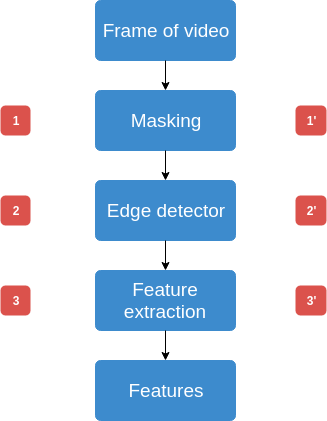
\includegraphics[width=2.5in]{_img/algorithm_overview.png}
\caption{Pattern detection pipeline.}
\end{figure}

\subsection{ Use of ROI }
We setted a ROI (Region Of Interest) based on the firsts iterations, after we extract enough features on \textit{Feature extraction} stage, we used a ROI based on coordinates in features and a margin for predicting next frame features in order to reduce processing and avoid noise produced by ambient.
\\
\\
\subsection{ Masking }
This step is in charge of isolating the pattern by using threhsolding operations.
\\
\\
The approach consists on creating a mask from the grayscale transformed image applying \textbf{Adaptive Thresholding algorithm}, this algorithm relies on Integral Image technique especified in \cite{IntegralImageThresholding}.
\\
\\
%% TODO: Gerson
\begin{algorithm}
\caption{Masking}
\label{alg:mask2}
\begin{algorithmic}[1]
\State $\textit{Set up thresholding parameters}$
\State $mask   = \textit{rgb2gray}( inputImage )$
\State $mask   = \textit{AdaptiveThreshold}(mask, blockSize)$\\
\Return $masked$
\end{algorithmic}
\end{algorithm}
%%%%%%%%%%%%%%%%%%%%%%%%%%%%%%%%%%%%%%%%%%%%%%%%%%%%%%%

\subsection{Edge detection}
In this stage of the pipeline we extract edges from the result of the previous stage. In order to do this, we applied \textbf{Scharr operators} on \textit{x} and \textit{y} axis (as described in algorithm 2); Scharr is the result from Sobel algorithm minimizing weighted mean squared angular error in Fourier domain.
%% TODO: Gerson
\begin{algorithm}
\caption{Edge detection}
\begin{algorithmic}[1]
\State $axis_x   = \textit{Scharr}(masked, 1, 0)$
\State $axis_x   = \textit{Abs}(axis_x)$
\State $axis_y   = \textit{Scharr}(masked, 0, 1)$
\State $axis_y   = \textit{Abs}(axis_y)$
\State $edgesImage   = \textit{Add}(axis_x, axis_y)$ \\
\Return $edgesImage$
\end{algorithmic}
\end{algorithm}
\\
\\
\subsection{Feature extraction}
The last stage consist of extracting the features needed for the calibration from the edges detected in the previous stage. We used OpenCV's \textbf{SimpleBlobDetector} that apply an extra thresholding on image, applies the findContours algorithm calculating their centers, groups centers of several images by their coordinates in blobs, finally, estimates the final centers of blobs. For detecting only pattern blobs, we had to apply similar heuristics to avobe (color blobs, area, aspect ratio, and convexity of points) specified in \textit{Algorithm 3}.
\\
\\
Also, in this stage we recognized the order of features detected. We started calculating the center of pattern given by the average coordinates of all features, then we computed features which are located in the corners of the pattern given by the farthest features from the center point. Next, we detected the vertical border points, selecting the nearest point to the line that pass through two corners. Similarly, we used border points to recognize the horizontal strips of points.
\\
\\ 
Finally, we used this information to give an ID number to every key point in pattern and store their location to track in next phase.
\\
\\
It should be noted that we only do recognition of features once, in next frames we only will extract features using \textit{SimpleBlobDetector} and track key points result in next step.
\\
\\
%% TODO: Gerson
\begin{algorithm}
\caption{Feature extraction}
\begin{algorithmic}[1]
\State $\textit{Set up detector parameters}$
\State $\textit{SimpleBlobDetector}(params)$
\State $keypoints   = \textit{detect}(mask)$ 
\State $midPt   = \textit{avg}(keypoints)$
\State $newKeypts[corners] = farthest(keypoints, midPt)$
\State $newKeypts[bord] = near(newKeypts[corners], keypoints)$
\State $newKeypts[rest] = near(newKeypts[bord], keypoints)$\\
\Return $newKeypts$
\end{algorithmic}
\end{algorithm}

\subsection{Tracking}
To track Feature Points extracted in previous phase, we compared stored keyPoints of the last frame and the new Keypoints of the current frame, we stored new positions using a range of movement and a delta that represents speed in movement between frames.
\\
\\
Also, when not all keypoints are detected in previous phase, we try to predice the position of the lost points using neighbors information (position and speed).
\\
\\


\section{Results}
We implemented the pipeline using the \textbf{OpenCV} library. The following images show some results of applying the approach to a video recording.

\begin{figure}[H]
\centering
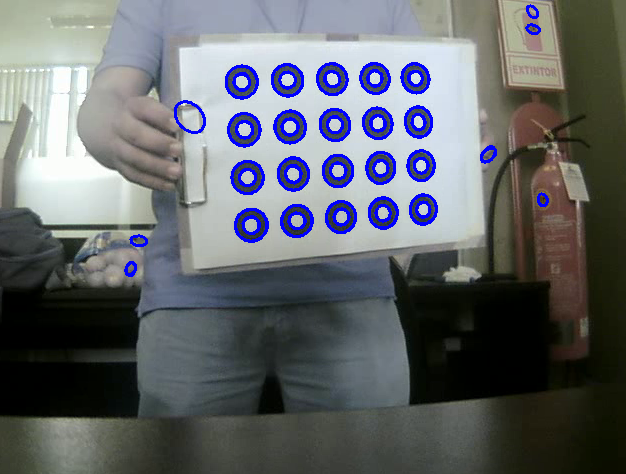
\includegraphics[width=2.5in]{_img/img_results_p1.png}
\caption{Results using pipeline 1.}
\end{figure}
%
\begin{figure}[H]
\centering
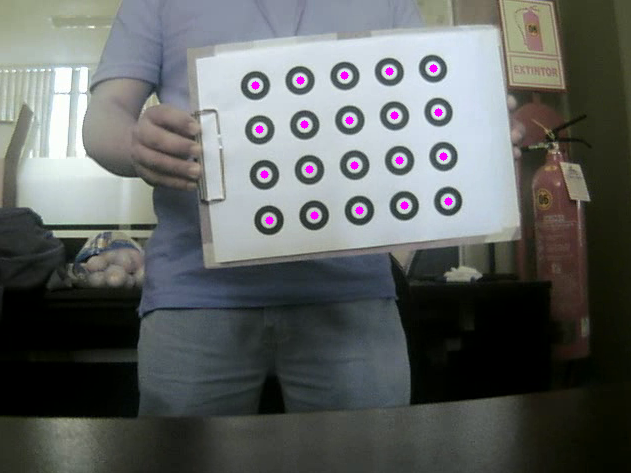
\includegraphics[width=2.5in]{_img/img_results_p2.png}
\caption{Results using pipeline 2.}
\end{figure}
%
\section{Conclusions and Future improvements}
The main issue in both pipeline implementations is that we are using just global information from each frame. This gives some acceptable results, but in cases where there is quite some changes in ilumination, the pipeline may break. In these situations, we could use the fact that the pattern is moving, as well as the fact that the pattern is fixed and the resulting centers should be in a grid like pattern in some way.
\\
\\
We plan on using object tracking, by using an initial estimation of the circles. To get an initial estimation we plan on isolating a region of interest manually, and then track the initial estimation using optical flow or some other techniques, as shown in the following figure.
\\
\begin{figure}[H]
\centering
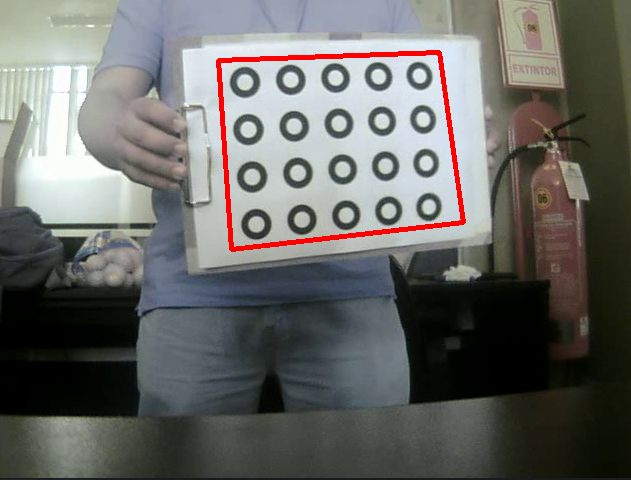
\includegraphics[width=2.5in]{_img/img_results_fut_1.png}
\caption{Initial estimation.}
\end{figure}
%
We plan on also use some fitting method to ensure that we can remove outliers from the grid pattern.

\IEEEtriggeratref{8}

% references section
\begin{thebibliography}{1}

\bibitem{OpenCV}
  Bradski, G. \\
  \textit{OpenCV library.} - 2000
\\
\bibitem{CameraCalibration1}
  Zhengyou Zhang \\
  \textit{A Flexible New Technique for Camera Calibration.} - 2000
\\
\bibitem{IntegralImageThresholding}
  Derek Bradley, Gerhard Roth \\
  \textit{Adaptive Thresholding Using the Integral Image.} - 2011


\end{thebibliography}


\end{document}


